%Rendering of the simplest possible Graph
\begin{figure}
    \begin{center}
        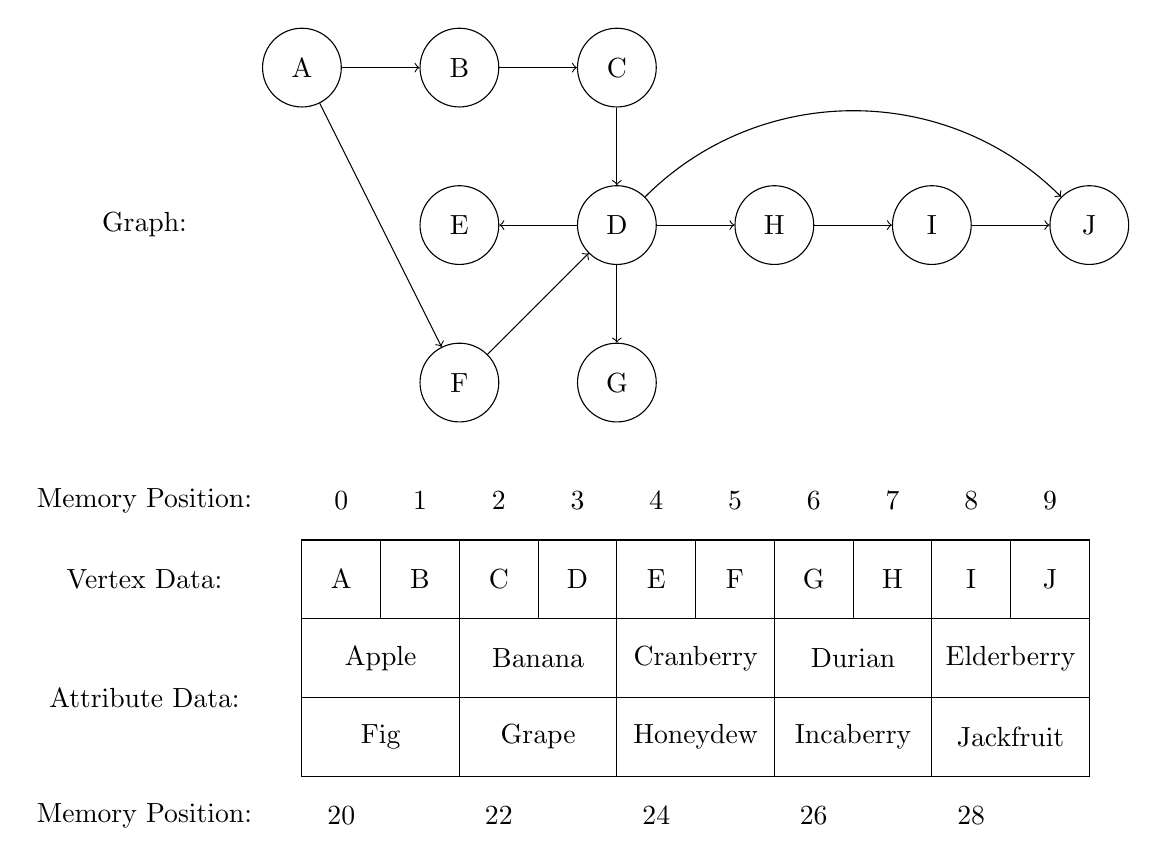
\begin{tikzpicture}

            % Graph vertices
            \node[circle,draw,minimum size=1cm] (A) at (0,0) {A};
            \node[circle,draw,minimum size=1cm] (B) at (2,0) {B};
            \node[circle,draw,minimum size=1cm] (C) at (4,0) {C};
            \node[circle,draw,minimum size=1cm] (D) at (4,-2) {D};
            \node[circle,draw,minimum size=1cm] (E) at (2,-2) {E};
            \node[circle,draw,minimum size=1cm] (F) at (2,-4) {F};
            \node[circle,draw,minimum size=1cm] (G) at (4,-4) {G};
            \node[circle,draw,minimum size=1cm] (H) at (6,-2) {H};
            \node[circle,draw,minimum size=1cm] (I) at (8,-2) {I};
            \node[circle,draw,minimum size=1cm] (J) at (10,-2) {J};
            
            % Graph Edges
             \draw[->] (A) -- (B);
             \draw[->] (A) -- (F);
             \draw[->] (B) -- (C);
             \draw[->] (C) -- (D);
             \draw[->] (D) -- (E);
             \draw[->] (F) -- (D);
             \draw[->] (D) -- (G);
             \draw[->] (D) -- (H);
             \draw[->] (D) to [out=45,in=135] (J);
             \draw[->] (H) -- (I);
             \draw[->] (I) -- (J);

            %Memory Array
             \foreach \x/\letter in {0/A, 1/B, 2/C, 3/D, 4/E, 5/F, 6/G, 7/H, 8/I, 9/J} {
                
                \node at (\x+0.5, -5.5) {\x};
                \draw (\x,-7) rectangle ++(1,1);
                \node at (\x+0.5, -6.5) {\letter};
                
             }

            %Attribute Array:

            \foreach \x/\attr in {0/Apple, 2/Banana, 4/Cranberry, 6/Durian, 8/Elderberry} {
                % \node at (\x,-8) {1\x};
                \draw (\x,-8) rectangle ++(2,1);
                \node at (\x+1,-7.5) {\attr};
            }
            \foreach \x/\attr in {0/Fig, 2/Grape, 4/Honeydew, 6/Incaberry, 8/Jackfruit}{
                \draw (\x,-9) rectangle ++(2,1);
                \node at (\x+1,-8.5) {\attr};
                \node at (\x+0.5,-9.5) {2\x};
            }
            
            %Labels
            \node at (-2,-2) {Graph:};
            \node at (-2,-5.5) {Memory Position:};
            \node at (-2,-6.5) {Vertex Data:};

            \node at (-2, -8) {Attribute Data:};
            \node at (-2, -9.5) {Memory Position:};


            \end{tikzpicture}
        \caption{A simplified representation of a directed graph in vertex order where each vertex is added to memory creation order with attributes stored separately. Pointers from topology to attributes are not shown for clarity but correspond to the first letter of the attribute.}
        \label{figure:locality-attributed}          
    \end{center}
\end{figure}